% Minkowski's convex body theorem: a symmetric convex body of area > 4 covol contains a non-zero lattice point (generated).
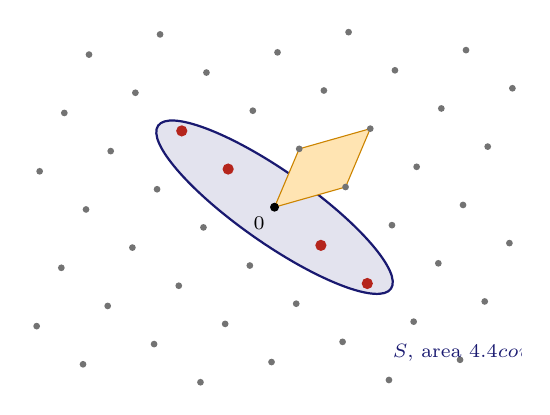
\begin{tikzpicture}[scale=0.95]
\clip (-3.3,-2.4) rectangle (3.3,2.4);
\fill[MidnightBlue!12,draw=MidnightBlue,thick,rotate=-35.0] (0,0) ellipse (1.900 and 0.481);
\fill[Orange!30,draw=Orange!80!black] (0,0)--(0.95,0.27)--(1.28,1.05)--(0.33,0.78)--cycle;
\fill[black!55] (-3.140,0.480) circle (0.045);
\fill[black!55] (-2.810,1.260) circle (0.045);
\fill[black!55] (-2.480,2.040) circle (0.045);
\fill[black!55] (-3.180,-1.590) circle (0.045);
\fill[black!55] (-2.850,-0.810) circle (0.045);
\fill[black!55] (-2.520,-0.030) circle (0.045);
\fill[black!55] (-2.190,0.750) circle (0.045);
\fill[black!55] (-1.860,1.530) circle (0.045);
\fill[black!55] (-1.530,2.310) circle (0.045);
\fill[black!55] (-2.560,-2.100) circle (0.045);
\fill[black!55] (-2.230,-1.320) circle (0.045);
\fill[black!55] (-1.900,-0.540) circle (0.045);
\fill[black!55] (-1.570,0.240) circle (0.045);
\fill[BrickRed] (-1.240,1.020) circle (0.075);
\fill[black!55] (-0.910,1.800) circle (0.045);
\fill[black!55] (-1.610,-1.830) circle (0.045);
\fill[black!55] (-1.280,-1.050) circle (0.045);
\fill[black!55] (-0.950,-0.270) circle (0.045);
\fill[BrickRed] (-0.620,0.510) circle (0.075);
\fill[black!55] (-0.290,1.290) circle (0.045);
\fill[black!55] (0.040,2.070) circle (0.045);
\fill[black!55] (-0.990,-2.340) circle (0.045);
\fill[black!55] (-0.660,-1.560) circle (0.045);
\fill[black!55] (-0.330,-0.780) circle (0.045);
\fill[black] (0,0) circle (0.06) node[below left,font=\scriptsize]{$0$};
\fill[black!55] (0.330,0.780) circle (0.045);
\fill[black!55] (0.660,1.560) circle (0.045);
\fill[black!55] (0.990,2.340) circle (0.045);
\fill[black!55] (-0.040,-2.070) circle (0.045);
\fill[black!55] (0.290,-1.290) circle (0.045);
\fill[BrickRed] (0.620,-0.510) circle (0.075);
\fill[black!55] (0.950,0.270) circle (0.045);
\fill[black!55] (1.280,1.050) circle (0.045);
\fill[black!55] (1.610,1.830) circle (0.045);
\fill[black!55] (0.910,-1.800) circle (0.045);
\fill[BrickRed] (1.240,-1.020) circle (0.075);
\fill[black!55] (1.570,-0.240) circle (0.045);
\fill[black!55] (1.900,0.540) circle (0.045);
\fill[black!55] (2.230,1.320) circle (0.045);
\fill[black!55] (2.560,2.100) circle (0.045);
\fill[black!55] (1.530,-2.310) circle (0.045);
\fill[black!55] (1.860,-1.530) circle (0.045);
\fill[black!55] (2.190,-0.750) circle (0.045);
\fill[black!55] (2.520,0.030) circle (0.045);
\fill[black!55] (2.850,0.810) circle (0.045);
\fill[black!55] (3.180,1.590) circle (0.045);
\fill[black!55] (2.480,-2.040) circle (0.045);
\fill[black!55] (2.810,-1.260) circle (0.045);
\fill[black!55] (3.140,-0.480) circle (0.045);
\node[font=\scriptsize,MidnightBlue,anchor=west] at (1.45,-1.95) {$S$, area $4.4\operatorname{covol}(L)$};
\end{tikzpicture}
